\def\year{2015}
%File: formatting-instruction.tex
\documentclass[letterpaper]{article}
\usepackage{aaai}
\usepackage{times}
\usepackage{helvet}
\usepackage{courier}
\usepackage{graphicx}
\usepackage{float}
\usepackage{subfig}
\usepackage{pgfplotstable}
\usepackage{pgfplots}
\usepackage{nameref}
\usepackage{txfonts}
\frenchspacing
\setlength{\pdfpagewidth}{8.5in}
\setlength{\pdfpageheight}{11in}
\pdfinfo{
/Title (Using Domain Knowledge to Improve Monte-Carlo Tree Search Performance in Parameterized Poker Squares)
/Author (Robert Arrington, Clay Langley, Steven Bogaerts)}
\setcounter{secnumdepth}{0}  
 \begin{document}
% The file aaai.sty is the style file for AAAI Press 
% proceedings, working notes, and technical reports.
%
\title{Using Domain Knowledge\\To Improve Monte-Carlo Tree Search Performance\\In Parameterized Poker Squares}    % ***** DON'T FORGET TO PUT TITLE IN THE METADATA ABOVE TOO!
\author{Robert Arrington, Clay Langley, Steven Bogaerts\\
Department of Computer Science\\
DePauw University\\
Greencastle, IN, USA\\
\{{\tt robertarrington\_2015}, {\tt claylangley\_2017}, {\tt stevenbogaerts}\}{\tt@depauw.edu}
}
\maketitle
\begin{abstract}
\begin{quote}
Poker Squares is a single-player card game played on a 5 x 5 grid, in which a player attempts to create as many high-scoring Poker hands as possible. As a stochastic single-player game with an extremely large state space, this game offers an interesting area of application for Monte-Carlo Tree Search (MCTS). This paper describes enhancements made to the MCTS algorithm to improve computer play, including pruning in the selection stage and a greedy simulation algorithm. These enhancements make extensive use of domain knowledge in the form of a state evaluation heuristic. Experimental results demonstrate both the general efficacy of these enhancements and their ideal parameter settings.
\end{quote}
\end{abstract}

%%%%%%%%%%%%%%%%%%%%%%%%%%%%%%%%%%%%%%%%%%%%%%%%%%%%%%%%%
\section{Introduction}

Poker Squares is a single-player card game played on a 5~x~5 grid, on which the player places one drawn card at a time. Once placed, a card may not be moved. The goal is to create as many high-scoring Poker hands as possible in each of the five rows and five columns. Due to the overlapping of rows and columns and the uncertainty of what cards will be drawn in what order, players must balance the risk of pursuing high-scoring hand types with the safer but less-rewarding pursuit of more easily-attained hand types.

In human play, two of the most common scoring systems are American and British (Table~\ref{tbl:scoring}). {\it Parameterized} Poker Squares (PPS) includes the added challenge that the player is not told the scoring system until the moment the game begins. So the scoring system may be standard American or British, or perhaps a system in which positive points are given for a full house and negative points for all other hand types, or even a random scoring system (Table~\ref{tbl:scoring}). Thus the player must be highly adaptive.

%\begin{figure}[b]
%\begin{center}
%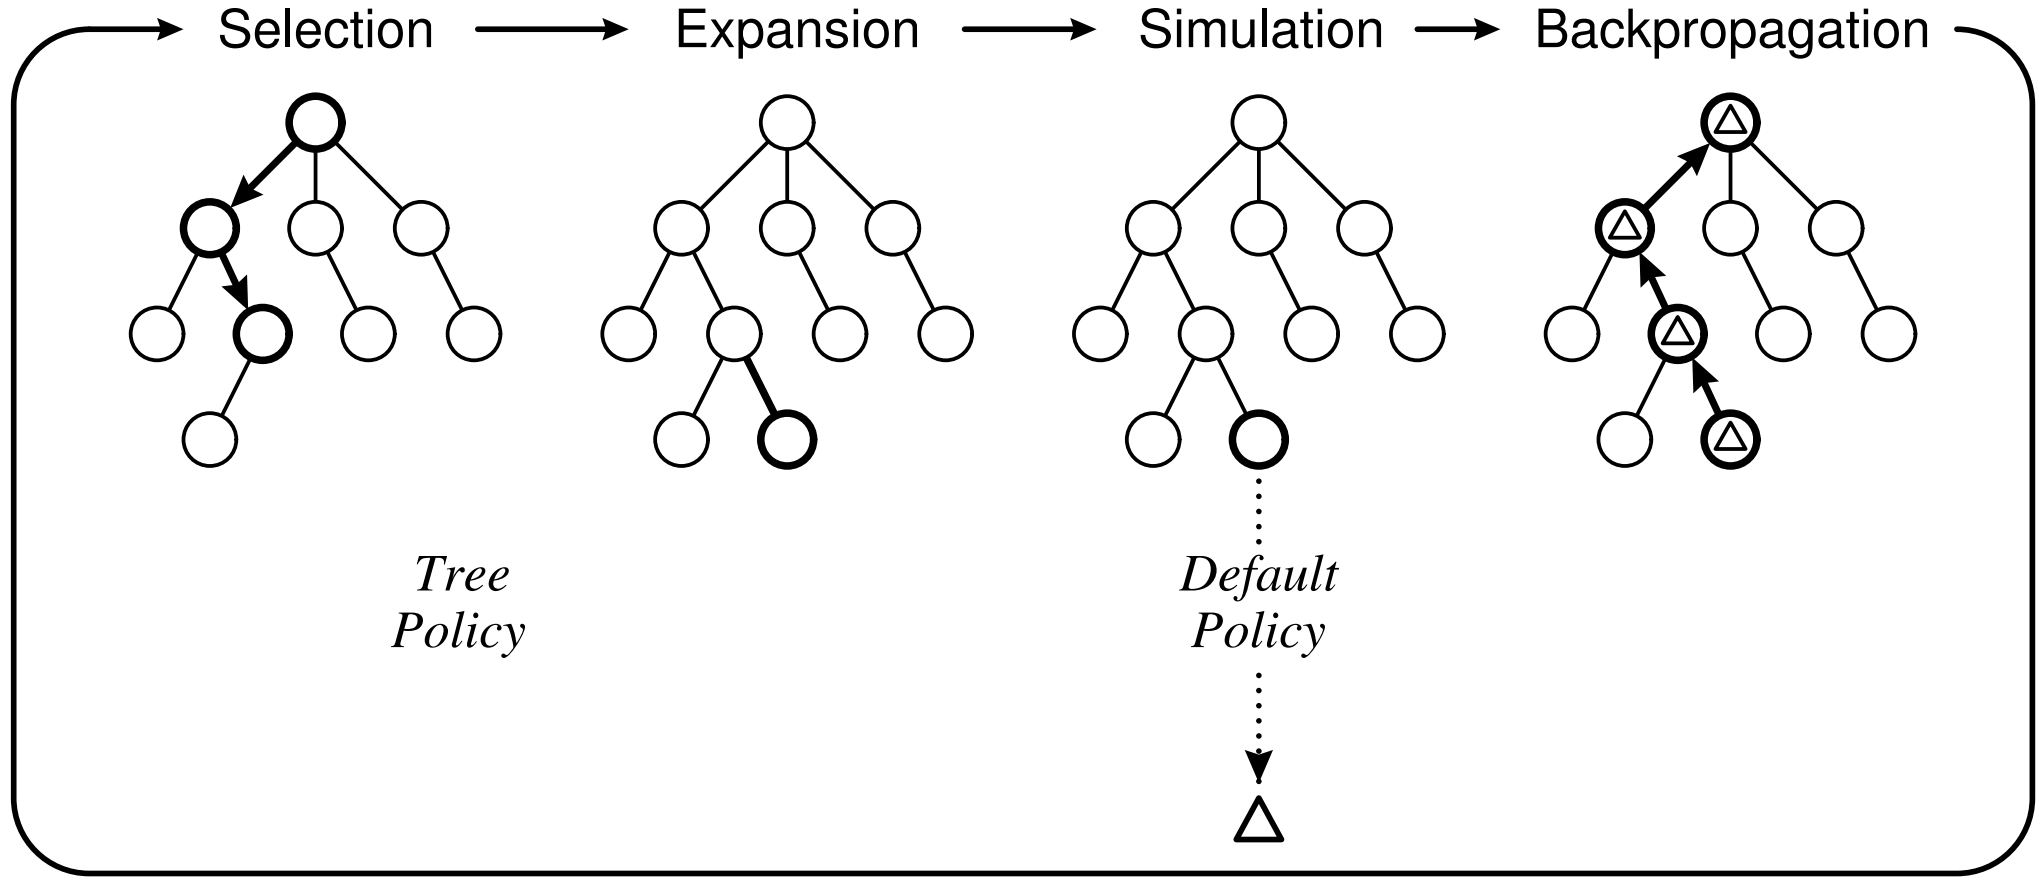
\includegraphics[width=.95\linewidth]{images/oneiteration.png}
%\end{center}
%\caption{Outline of MCTS~\cite{browne2012survey} }
%\label{fig:OneIter}
%\end{figure}

This paper considers the application of Monte-Carlo Tree Search (MCTS) to PPS. Like other game-playing algorithms, at its core MCTS involves the creation of a game tree to decide on a move. MCTS is typically applied to games with extremely large trees, because the algorithm is designed to build the tree selectively rather than exhaustively. This paper begins with a brief introduction to MCTS, followed by a discussion of related work, key enhancements to MCTS to play this game, experiments showing the effectiveness and ideal use of these enhancements, and future work.

\begin{table}
\caption{Example scoring systems}
\label{tbl:scoring}
\centering
\begin{tabular}{r r r r r}
\hline
\multicolumn{1}{c}{\textbf{Hand Type}} & 
\multicolumn{1}{c}{\textbf{Am.}} & 
\multicolumn{1}{c}{\textbf{Brit.}} & 
\multicolumn{1}{c}{\textbf{F.H.}} & 
\multicolumn{1}{c}{\textbf{Random}} \\
\hline
royal flush     & 100 & 30 & -1 & -23 \\
straight flush & 75 & 30 & -1 & -55 \\
4 of a kind    & 50 & 16 & -1 & 32 \\
straight        & 25 & 10 & -1 & -64 \\
full house     & 20 & 5  & 1 & -102 \\
3 of a kind   & 15 & 12 & -1 & 16 \\
flush           & 10 & 6   & -1 & 118 \\
2 pair         & 5   & 3   & -1 & -126 \\
1 pair         & 2   & 1   & -1 & 11 \\
high card    & 0   & 0   & -1 & -128 \\
\hline
\end{tabular}
\end{table}


%%%%%%%%%%%%%%%%%%%%%%%%%%%%%%%%%%%%%%%%%%%%%%%%%%%%%%%%%
\section{Monte-Carlo Tree Search}

The four-state process of MCTS consists of selection, expansion, simulation, and backpropagation. The {\it selection} step balances goals of exploration and exploitation to select a node for further consideration. Briefly, a measure of the most ``interesting'' child of a given node is applied recursively from the root down the tree to some not-fully-expanded descendant node. One common measure of the most ``interesting'' child is the upper-confidence bound applied to trees (UCT)~\cite{kocsis2006improved}, in which a child $j$ is chosen to maximize:

\begin{equation} \label{eq:UCT}
UCT = \overline{X}_j + 2C_p\sqrt{\frac{2\ln{n}}{n_j}}
\end{equation}

\noindent where $\overline{X}_j$ is the mean score obtained in games passing through child $j$, $n$ is the number of visits to the parent node during tree construction, $n_j$ the number of visits to child $j$, and $C_p > 0$ is a constant. Thus the $\overline{X}_j$ term is the {\it exploitation} term, through which children with higher average scores will receive higher UCT scores, and therefore be more likely selected for further consideration. Similarly, the second term is the {\it exploration} term, in which a child that has been visited significantly less frequently than the parent will receive a higher UCT score. Therefore, $C_p$ balances the goals of exploitation and exploration in selecting a child of a given node. Again, UCT can be applied recursively starting at the root to traverse to a not-fully-expanded node in the existing tree, thus completing the {\it selection} stage.

In {\it expansion}, a previously unconsidered child $v$ of the selected node is randomly selected. In {\it simulation}, a game is played from $v$ to completion; in standard MCTS, simulation consists entirely of random moves. Finally, in {\it backpropagation}, results of the simulation are used to update all nodes on the path from $v$ up to the root: each node's visit count $n$ is incremented and average score $Q$ is updated based on the result of the simulated game. In this way, the tree is gradually and selectively developed, providing an increasingly detailed picture of the expected score from various states in the state space. Upon reaching some limit condition, a child of the root can be selected based on any of a number of criteria, such as highest $Q$ or highest $n$. For a detailed discussion of the MCTS algorithm, see~\cite{browne2012survey}.

%%%%%%%%%%%%%%%%%%%%%%%%%%%%%%%%%%%%%%%%%%%%%%%%%%%%%%%%%
\section{Related Work In MCTS}
\label{relatedWork}

%PPS includes uncertainty in the drawing of cards. One common approach for handling uncertainty is through the use of both {\it chance} and {\it choice} nodes \cite{melko2007optimal,hauk2004search}. In this approach, choice nodes can be treated as usual, while chance nodes can be selected randomly rather than using UCT.

Much prior work in MCTS has applied pruning to the game tree. In {\it soft pruning}, a suboptimal node is hidden from consideration, but can be brought back if warranted by later re-evaluation. In contrast, {\it hard pruning} offers no possibility for bringing a pruned node back~\cite{browne2012survey}. Most commonly, the node's $Q$ value is used in making pruning decisions, but \cite{huang2010pruning} describe alternative soft (``relative'') and hard (``absolute'') pruning techniques based on the visit count $n$.

Additional pruning strategies using domain knowledge have been applied to the multi-player card game Lords of War~\cite{sephton2014ieee}. In this work, state evaluations based on card counting are used to prune states that are less likely to be useful. This work also considers the additional time required for such evaluations -- time that could be spent further exploring the tree. Significant improvements are obtained with pruning despite this trade-off.

Simulation strategies enhanced with domain knowledge have also been useful in MCTS research. For example, in \cite{winands2010monte} an MCTS player for the strategy game Lines of Action uses a simulation that was cut short, backpropagating a heuristic evaluation prior to the end of the game rather than playing to completion. Another approach is to use a heuristic to guide simulation, rather than choosing moves randomly. For example, \cite{schadd2012single} reports a 50\% increase in average score in the game SameGame when an accurate heuristic was added.

%%%%%%%%%%%%%%%%%%%%%%%%%%%%%%%%%%%%%%%%%%%%%%%%%%%%%%%%%
\section{MCTS Application to PPS}

%\begin{table}
%\caption{Scoring Systems: Ameritish and a random.}
%\label{tbl:SSATRD}
%\centering
%\begin{tabular}{c c c}
%\hline
%Hand & Ameritish & Random \\
%\hline
%royal flush & 47 & -23 \\
%straight flush & 47 & -55 \\
%4 of a kind & 24 & 32 \\
%straight & 13 & -64 \\
%full house & 9 & -102 \\
%3 of a kind & 8 & 16 \\
%flush & 6 & 118 \\
%2 pair & 4 & -126 \\
%1 pair & 1 & 11 \\
%high card & 0 & -128 \\
%\hline
%\end{tabular}
%\end{table}

Our MCTS application to PPS is built on top of the code in~\cite{hughart2012uct}, used under the MIT software license. The MCTS algorithm is run each time a move is needed. The tree begins with a choice node at its root, in which the current card must be placed in the grid. The children are chance nodes, representing the random drawing of the next card to be played, with alternating choice and chance nodes through the remaining levels of the tree. This tree is gradually and selectively developed by repeatedly executing the four stages of MCTS, with UCT in the selection stage. We limit each game to 30 seconds in total, both to make significant experimentation more manageable, and to maintain eligibility for an upcoming PPS computer player contest. 

For the first, second, next-to-last, and last moves, some simple rules are used rather than the full MCTS process. For the remaining moves, our ``core'' implementation of MCTS uses no domain knowledge in selection nor simulation. We describe next some enhancements on this core application of MCTS, in which domain knowledge is added to both selection and simulation. This is followed by a discussion of experimental results for these enhancements.

\subsection{Domain Knowledge}

While one benefit of the core MCTS algorithm is that very little domain knowledge is required, nevertheless great performance improvements can be obtained with additional knowledge. This subsection describes a PPS state-evaluation heuristic, with the following subsections describing its application to simulation and selection.

A state is evaluated by adding the scores of each of its ten Poker hands. Thus a state-evaluation heuristic is the sum of ten applications of a hand-evaluation heuristic. When the hand in question contains five cards, the system must simply determine what hand type is represented, and look up the corresponding score for the current scoring system.

For hands containing one to four cards, we first calculate a {\it possibility array}. This array contains one slot for each hand type, from high card to royal flush. In each slot, $0$ indicates that the hand type is no longer possible, $1$ indicates the hand type is possible, and $2$ indicates the hand type is already made. For example, if a hand contains one card only, then high-card is $2$ and all other elements are $1$, except that royal flush may be $0$ if the card is lower than ten and not an ace. If a second card placed in the hand produces a pair, then high-card and any hand types involving a straight would become $0$, while pair would become $2$. In turn, as more cards are added, additional hand types may become impossible.

Four-card hands use the possibility array in a different way than do one-, two-, and three-card hands. For each of the hand types, a {\it weight} in $[0,1]$ is calculated, representing a rough measure of the likelihood of obtaining that hand type with the next card draw. For a hand type with a 0 in the possibility array, the weight is set to 0. For a hand type with a 1 in the possibility array, the cards remaining in the deck are analyzed to determine the weight. For example, if a hand needs a $10\varheartsuit$ or $10\clubsuit$ to complete a full house, and the remaining cards in the deck include a $10\varheartsuit$ and five different $\spadesuit$ cards, then the weight for a full house is calculated as $1 / 6$. 

For a hand type with a 2 in the possibility array (a hand type that has already been achieved), the weight is not necessarily set to 1. For example, suppose a 4-card hand contains a $6\varheartsuit$, $6\clubsuit$, $6\spadesuit$, and $7\spadesuit$, while the deck contains only a $6\vardiamondsuit$, $7\varheartsuit$, and $8\varheartsuit$. Here, the weight of three-of-a-kind, four-of-kind, and full house would all be $1/3$, since one of the three remaining cards in the deck leads to each of these hand types.

Once these weights are calculated for every hand type, each weight is multiplied by the hand type value according to the current scoring system, and added together to form a weighted sum. Note that these calculations ignore the fact that the ten hands in the grid are dependent on each other. This dependence is due to overlap of the rows and columns on the grid, and occasional ``competition'' between hands for the same card. Nevertheless, this calculation gives a reasonable heuristic for the evaluation of four-card hands.

This approach gets much more computationally intensive for hands with fewer than four cards, and so in this case we instead use {\it a-priori} probabilities of hand types as weights. We developed these a-priori probabilities from the British scoring system for Poker Squares, which is based on the difficulty of finishing each of the hand types. (Note that Poker Squares probabilities are not the same as Poker probabilities.) These probabilities are then used to compute a weighted sum in the same way as in a four-card hand.

These calculations can readily accommodate any scoring system as a parameter. For example, if three-of-a-kind is valued at -100 points, then a high weight for three-of-a-kind would lead to a significant drop in the weighted sum. Thus this heuristic is highly adaptive to any scoring system.

Note, however, that there should be some value distinction between one-, two-, and three-card hands. For example, a one-card hand will have nearly all, if not all, hand types listed as ``possible'' in the possibility array. A two-card hand will likely list fewer hand types as possible, and a three-card hand fewer still. Yet a three-card hand is closer to completing its possible hand types than is a two- or one-card hand, even with the same values in the possibility array. So all else being equal, a three-card hand should be weighted more highly. To account for this, we apply weights $\alpha$, $\beta$, and $\gamma$ for one-, two-, and three-card hands, respectively. While we would expect that $0 < \alpha < \beta < \gamma < 1$, ideal values are the subject of  experiments described later. In an initial implementation, we fix these values at $\alpha = 0.2$, $\beta = 0.4$, and $\gamma = 0.6$.

\subsection{Modified Selection Through Pruning}

Recall in our core MCTS implementation that the selection process uses UCT to find a not-fully-expanded node. This means that nodes with low visit counts are favored, to some extent even when observed rewards are low. While some other games do have significantly higher branching factors than PPS, there is still potentially much to gain through pruning. The state heuristic can be used for this purpose.

As discussed in the section {\it \nameref{relatedWork}}, there are two typical strategies for pruning: soft pruning, in which pruned nodes may be brought back, and hard pruning, in which pruned nodes are lost forever. While soft pruning may have some benefits, the decision of whether or not to bring a node back leads to extra computation and knowledge requirements, and so we opt for hard pruning in this work.

First we calculate the heuristic score $h(p)$ for the parent. The value $\delta \cdot h(p)$, for some constant $\delta$, is set as the heuristic score threshold for each child. All children below this threshold are pruned, never to be considered for selection. For example, $\delta = 0.9$ would prune children with $ < 90\%$ of the score of the parent, while any $\delta > 1$ would prune all children that do not improve over the score of the parent. For the purposes of future experiments, we fix $\delta$ at $1.30$.

In practice, this sometimes leads to over-pruning. For example, if a drawn card does not fit well in any open space, all children may have lower heuristic scores than the parent. Thus an additional safeguard is used, that no more than 70\% of the children of any given parent may be pruned. If the  $\delta \cdot h(p)$ threshold prunes more than this amount, then only the bottom 50\% of the children are pruned.

\subsection{Modified Simulation}

While the core MCTS implementation uses a completely random game in the simulation step, the state heuristic can also be applied to alternative simulation strategies. A {\it pruning simulation} strategy can apply the same pruning described above to simulation, such that a move is randomly chosen from among the non-pruned children. Alternatively, a {\it best move simulation} can be applied, in which all children are evaluated with the state heuristic, and the highest-scoring child is taken as the choice in simulation. The trade-off of these approaches, of course, is that they are more computationally-intensive, and thus fewer iterations of the MCTS process can be completed in a given time period. 

%%%%%%%%%%%%%%%%%%%%%%%%%%%%%%%%%%%%%%%%%%%%%%%%%%%%%%%%%
\section{Experiments and Analysis}

The modifications to the core MCTS algorithm described in the previous section are evaluated experimentally here. We begin with a discussion of the exploration-exploitation trade-off, followed by the use of domain knowledge in both simulation and selection.

%-----------------------------------------------------------------------------------------------------------------------------------------------------------------
\subsection{The Exploration--Exploitation Tradeoff}
Recall from equation (\ref{eq:UCT}) that MCTS with UCT attempts to balance the exploitation of relatively effective paths with the exploration of lesser-known paths. This balance is controlled via the constant $C_p$, where a higher value means a stronger emphasis on exploration. As discussed previously, ~\cite{kocsis2006improved} suggest that $C_p=1 / \sqrt{2}$ is ideal when rewards range in $[0,1]$. 

In some games, a reward range in $[0,1]$ is straightforward. For example, 0 could mean a loss, and 1 a win, or maximum and minimum possible scores could be translated to 0 and 1, respectively, to ``squash'' the scores.

Unfortunately in PPS, squashing to the $[0,1]$ range is not straightforward. To find the maximum score, for example, a first attempt might be to simply take ten times the maximum-scoring hand. For example, with the American scoring system (Table~\ref{tbl:scoring}), this would be 1,000. Of course it is not possible to have ten royal flushes in a $5\times5$ grid, due to the dependence between hands and the use of a single deck of cards. In fact, in the American scoring system, the maximum score is 725, corresponding to four royal flushes, a straight flush, and five four-of-a-kinds. In a more unusual scoring system, a different set of hands might be higher-scoring. So finding a maximum (or minimum) for squashing is not trivial.

Compounding this problem is the difference between the maximum possible score and the most likely scores. In some scoring systems, scores close to the maximum may be easy to achieve -- for example, in a scoring system in which only high-card is worth positive points. In others, however, typical scores may be far lower than the maximum. In the American scoring system, for example, while 725 is the maximum possible, scores in the 100's are much more common. Squashing to the $[0,1]$ range would mean that a score of 100 would become $0.138$, while a score of 150 would become $0.207$. So most scores would be in a tight range, leaving the rest of the range up to 1 rarely used. This may have unintended consequences in the UCT calculation, as nodes would look more similar than they should due to this squashing under an unrealistically high maximum possible score.

Nevertheless, we did create multiple squashing algorithms to compare performance of various $C_p$ values with and without squashing. {\it Precise} squashing calculates a precise minimum and maximum score in order to squash exactly to the $[0,1]$ range. Since this method is not trivial across scoring systems, a faster yet less accurate {\it imprecise} squashing method was also developed, in which the lowest possible hand score was multiplied by 10 for the minimum, and the highest hand score multiplied by 10 for the maximum. In testing the American scoring system, we also examined a simple hard-coded maximum of 200, and as a test in absurdity, another squashing method using a maximum of 2,000 (2.76 times higher than the actual maximum of 725).

Each of these squashing mechanisms was tested with core MCTS by playing 700 games using the American scoring system. $C_p$ was set to $1 / \sqrt{2}$ as recommended for scores in the $[0,1]$ range. Results are shown in Table~\ref{tbl:Squashing}. The table demonstrates minimal impact of squashing accuracy; even the absurd maximum of 2,000 achieved fairly comparable results. This suggests that a simple imprecise squashing method is sufficient.

\begin{table}
\captionof{table}{Effect of Score Squashing}
\label{tbl:Squashing}
\centering
\begin{tabular}{r l r}
\hline
{\bf Method} & {\bf Range} & {\bf Score} \\
\hline
Precise & 0 -- 725 & 91 \\
Imprecise & 0 -- 1000 & 91 \\
Max 200 & 0 -- 200 & 90 \\
Max 2000 & 0 -- 2000 & 90 \\
\hline
\end{tabular}
\end{table}

%\begin{table}
%\captionof{table}{Effect of $C_p$ Values With No Squashing}
%\label{tbl:noSquashing}
%\centering
%\begin{tabular}{c c || c c}
%\hline
%{\bf $C_p$} & {\bf Mean Score} & {\bf $C_p$} & {\bf Mean Score} \\
%\hline
%0 & 15 &                                        50 & 93        \\
%$1 /\!\sqrt{2}$ & 64 &                      100 & 92                       \\
%5 & 90 &                                        $200 /\!\sqrt{2}$ & 91       \\
%10 & 93 &                                      6000 & 92        \\
%25 & 94 \\
%%1500 & 91 \\
%%3000 & 93 \\
%%6000 & 92 \\
%%10000 & 93 \\
%\hline
%\end{tabular}
%\end{table}

This begs the question, however, of whether squashing and using $C_p = 1 / \sqrt{2}$ is worthwhile at all. To explore this, we tested various $C_p$ values without squashing on the American scoring system. As shown in Figure~\ref{fig:Cp}, the lowest $C_p$ values have the worst results. For the American scoring system, at around 7.5, scores level off for the most part, with a slight peak score of 95 around $C_p = 20$. Pushing $C_p$ values even higher leads to only a slight reduction in score; even $C_p = 5000$ (not shown in the figure) earned a mean score of 91 in the American scoring system. This can be explained by noting that for any sufficiently high $C_p$ value, the exploration term of equation~\ref{eq:UCT} will dominate the exploitation term, and so further increases in $C_p$ have little effect.

It is also interesting to note that the best scores in Figure~\ref{fig:Cp} are a bit higher than the scores in Table~\ref{tbl:Squashing}. This is likely due to the issues described previously, that in games that do not use the full range of scores, squashing can be problematic. While the squashing procedure could likely be tuned precisely to achieve a higher score, it seems simpler in this case to achieve the same by adjusting the single variable $C_p$.

The goal of these experiments was to fix a $C_p$ value for the experiments that follow. Figure~\ref{fig:Cp} suggests that around $C_p = 20$ is the best value for American scoring. Since other scoring systems will have different typical scores, the ideal setting will vary by system. Figure~\ref{fig:Cp} does suggest, however, that reasonably good performance can be achieved for any $C_p$ value above some minimum dependent on the scoring system. Since we are designing a player to be effective under any system, we choose a fairly high $C_p = 200 / \sqrt{2} = 141.4$ and focus on other parameters in the remainder of this paper, rather than creating a more dynamic $C_p$ at this time.\footnote{This value was originally chosen based on the idea that 200 is often considered a ``winning'' score in the American system, and thus we were comparing it to a squashed value of 1. In practice this value gave good results across scoring systems, and so its use was continued, although other values would be appropriate as well.} 

\begin{figure}[t]
\begin{center}
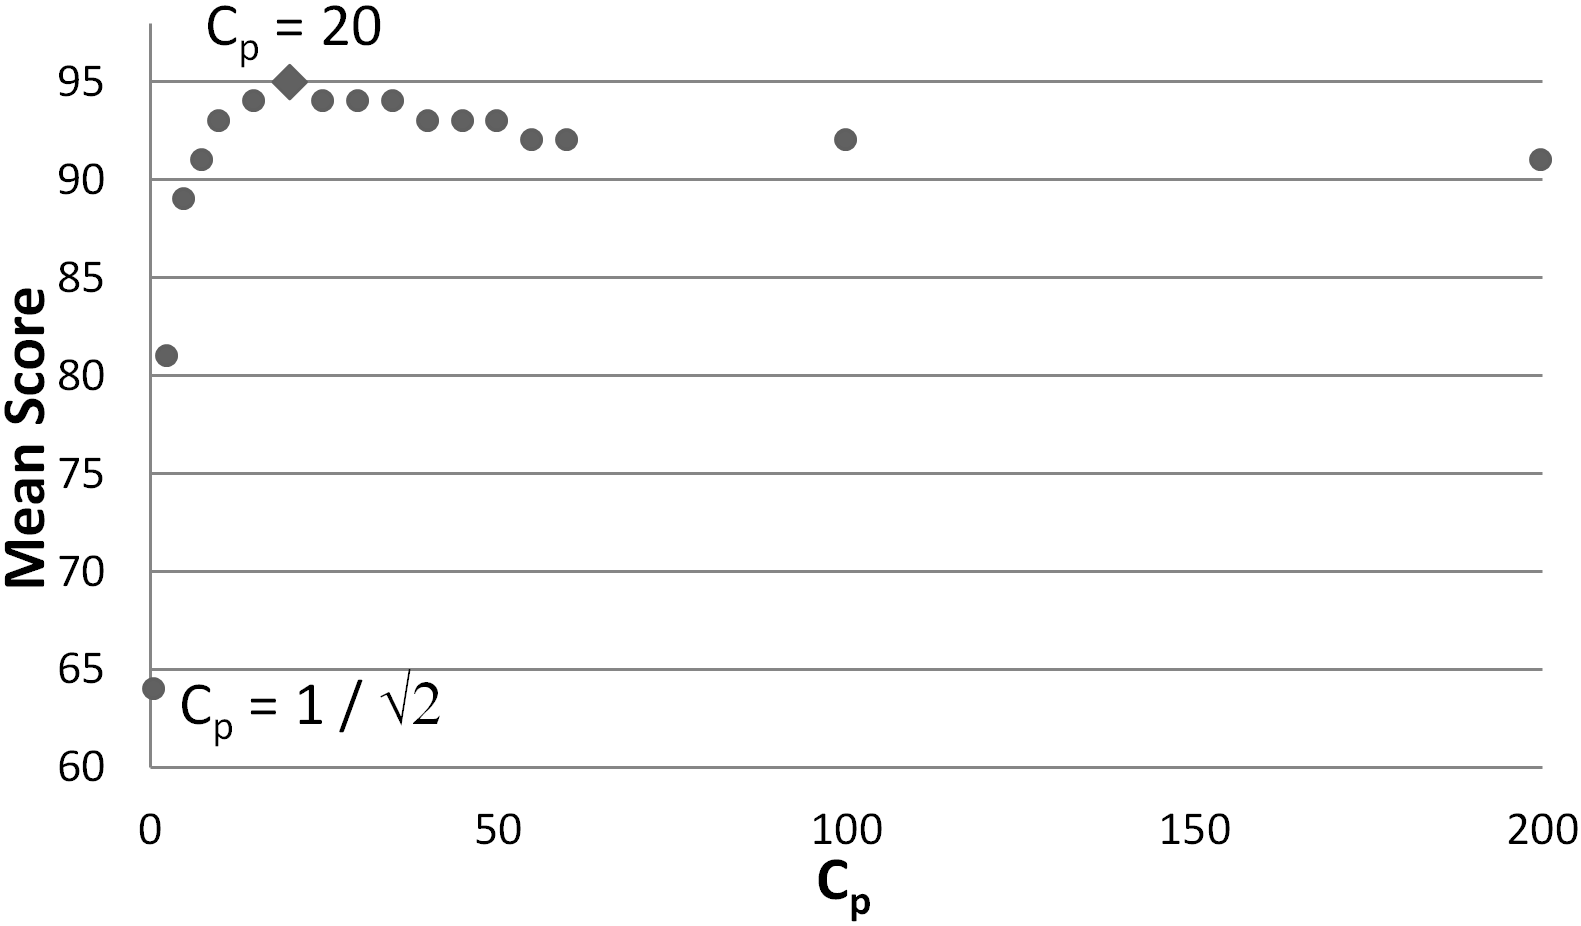
\includegraphics[width=1\linewidth]{images/Cp.png}
\end{center}
\caption{Mean score (American system) for various $C_p$}
\label{fig:Cp}
\end{figure}

%\begin{table}
%\captionof{table}{Effect of $C_p$ Values With No Squashing}
%\label{tbl:noSquashing}
%\centering
%\begin{tabular}{c c c}
%\hline
%{\bf $C_p$} & {\bf Mean Score} \\
%\hline
%0 & 15 \\
%$1 / \sqrt{2}$ & 64 \\
%5 & 90 \\
%10 & 93 \\
%25 & 94 \\
%50 & 93 \\
%100 & 92 \\
%$200 / \sqrt{2}$ & 91 \\
%%1500 & 91 \\
%%3000 & 93 \\
%%6000 & 92 \\
%10000 & 93 \\
%\hline
%\end{tabular}
%\end{table}

%\begin{figure}
%\begin{center}
%\begin{tikzpicture}
%\begin{axis}[width=.95\linewidth,    % was axis
%	xlabel=$C_P$,
%	ylabel=Mean Score, 
%	axis lines=left,
%	%xtick={0.00, 5.00, 10.00, 25.00, 50.00},
%	xmin=0, xmax = 60,
%	ytick={30.00, 60.00,90.00,120.0},
%	ymin=0, ymax = 100,
%	scaled y ticks = false,
%	y tick label style={/pgf/number format/fixed}]
%\addplot [only marks, mark size=1pt] table[y=mean_value, x=cp]{data/cpexperiment.dat};
%\end{axis}  % was axis
%\end{tikzpicture}
%\end{center}
%\caption{$C_p$: Effect of $C_p$ on Mean Score, no Squashing.}
%\label{fig:CPEXP}
%\end{figure}


%-----------------------------------------------------------------------------------------------------------------------------------------------------------------
\subsection{Computational Cost of the Heuristic}

As described above, the state-evaluation heuristic can be applied to create alternative selection and simulation strategies. Of course, heuristic calculations come at a computational cost, with more time required per iteration of the MCTS process, and therefore fewer iterations total in a given amount of time. So we start by examining the practical cost of the heuristic calculation itself.

We do this by considering heuristic {\it calculations} but not {\it applications} to any enhanced selection or simulation strategy. Table~\ref{tbl:SelSim} shows results for the American scoring system, with rows (1) -- (4) addressing the issue of heuristic calculation cost. Row (1) reflects standard MCTS, with UCT-based selection and random simulation. Rows (2) -- (4) also use these standard strategies, but with the ``+ Calc.'' notation indicating that the heuristic calculations are performed but not actually applied to any pruning or simulation enhancements. The drop in scores in rows (2) -- (4) compared to row (1) gives a reasonable indication of the cost of spending time on heuristic calculations rather than more iterations of MCTS. This deficit is 13 points (comparing rows (1) and (4)) in the American scoring system when the heuristic is calculated in both selection and simulation.

The data also show that the cost of adding calculations to selection is around just 1 or 2 points -- the difference between rows (3) and (4), and between rows (1) and (2), respectively. The cost of adding calculations to simulation, however, is much higher, at around 11 or 12 points -- the difference between rows (2) and (4), and between rows (1) and (3), respectively. This makes sense, as for each time that selection does the calculations, the simulation will do them several times -- once for every move in the remainder of the game. Thus any enhancement to selection or simulation must overcome the deficit of the added calculation cost before being worthwhile, with simulation enhancements having a much greater deficit to overcome than selection enhancements. The following subsections explore the extent to which some enhancements overcome this deficit.

\begin{table}
\captionof{table}{Selection and simulation results over 2,000 games}
\label{tbl:SelSim}
\centering
\begin{tabular}{rllr@{}l}
\hline
{\centering\bf Row} & {\centering\bf Selection} & {\centering\bf Simulation} & {\centering\bf Mean Score} & \\
\hline
\hline
(1) & UCT & Random & 92 \\
(2) & UCT + Calc. & Random & 90 \\
(3) & UCT & Random + Calc. & 80 \\
(4) & UCT + Calc. & Random + Calc. & 79 \\
\hline
(5) & UCT & Prune + Random & 95 \\
(6) & UCT & Best Move & 112 \\
\hline
(7) & Best Move & Random & 72 \\
(8) & Prune + UCT & Random & 91 \\
\hline
(9) & Prune + UCT & Best Move & 113 \\
\hline
(10) & Prune + UCT & Random & 94&\mbox{*}  \\
(11) & UCT & Best Move & 118&\mbox{*} \\
(12) & Prune + UCT & Best Move & 123&\mbox{*}  \\
\end{tabular}
\end{table}

%-----------------------------------------------------------------------------------------------------------------------------------------------------------------
\subsection{Domain Knowledge and Simulation}

%fixed: Simulation improvement using domain knowledge, but no pruning in selection
%variable: totally random simulation versus just choose the best move 
%result: choose best move is better

The state-evaluation heuristic can be used to create alternatives to random simulation. One such alternative, {\it prune + random} simulation, randomly selects each move not from the complete set of possible moves, but rather from a smaller set of nodes after pruning those scored beneath a threshold. The pruning technique used is the same as that previously described for selection. Another option is {\it best move} simulation, in which the highest-scoring move is always chosen.

Rows (1), (3), (5), and (6) of Table~\ref{tbl:SelSim} show the relevant results for these simulation experiments. Note prune + random simulation's mean score of 95 (row (5)) shows some improvement over the 92 of standard MCTS (row (1)). This is more striking when considering that prune + random's 95 actually overcame the drop down to 80 of the added heuristic calculation cost (row (3)).

Even more impressive, however, are the gains for best move simulation (row (6)). This approach earned a mean score of 112, significantly higher than the calculation deficit score of 80 (row (3)) and the standard MCTS score of 92 (row (1)). This demonstrates that, despite the added cost of the heuristic calculations, they are quite worthwhile in a best move simulation strategy.

It seems intuitive that best move simulation is more effective than prune + random, since best move plays a simulated game according to the best choices that the heuristic is capable of suggesting. In contrast, prune + random gives the heuristic less control, only determining a set of higher-scoring moves from which a random selection is made.

%\begin{table}
%\captionof{table}{Effect of Domain Knowledge on Simulation}
%\label{tbl:Simulate}
%\centering
%\begin{tabular}{c c c}
%\hline
%ID & Sim. Method & Mean Score \\
%\hline
%(1) & Random w/ Calc. & 81 \\
%(2) & Random w/o Calc. & 91 \\
%(3) & Best-Move & 118 \\
%\hline
%\end{tabular}
%\end{table}

%-----------------------------------------------------------------------------------------------------------------------------------------------------------------
\subsection{Domain Knowledge and Selection}

%fixed: Pruning in selection, with just some "sensible" weights
%variable: pruning just in selection with random sim vs. pruning in selection and simulation vs. pruning in selection and choose best sim.
%result: choose best move is better, and also we see the pruning in selection is helpful
%

This next set of experiments considers the application of the state heuristic to the selection step of MCTS. We consider {\it best move} selection, in which only the best child (according to the heuristic) is available for selection. We also consider {\it prune + UCT} selection, in which the heuristic is used to prune children below a threshold as described previously.

Consider again Table~\ref{tbl:SelSim}. Row (7) shows that with a score of 72, best move selection is highly ineffective, scoring even worse than row (2) in which the calculations are performed but not applied. This is not surprising, since such a drastic approach severely limits the number of nodes available for exploration. While best move {\it simulation} is a useful limitation in contrast to {\it random} simulation, the more principled exploration of {\it selection} with {\it UCT} should not be so severely restricted by a best move approach.

With a mean score of 91 (row (8)), prune + UCT selection shows little improvement over the non-application of the calculations (90 in row (2)) and a slight loss compared to standard MCTS (92 in row (1)). However, it is also interesting to consider rows (6) and (9). Using best move simulation instead of random simulation, there is a 1 point increase, rather than decrease, in using prune + UCT selection. Taken together, these results lead us to conclude that the application of prune + UCT as defined here is a wash -- the benefit is approximately equivalent to the cost. We will return to this issue and show slight improvement with a more tuned prune + UCT in the final set of experiments.

%\begin{table}
%\captionof{table}{Effect of Domain Knowledge on Selection}
%\label{tbl:Selection}
%\centering
%\begin{tabular}{c c c c}
%\hline
%ID & Sel. Method & Sim. Method & Mean Score \\
%\hline
%(4) & Best-Move & Best-Move & 84 \\
%(5) & Pruning & Random & 89 \\
%(6) & Pruning & Pruning & 107 \\
%(7) & Pruning & Best-Move & 120 \\
%\hline
%\end{tabular}
%\end{table}

%-----------------------------------------------------------------------------------------------------------------------------------------------------------------
\subsection{Further Tuning of Domain Knowledge}

%fixed: pruning in selection, choose best move for simulation
%variable: the weights for the board score
%result: the best weights we came up with

 %Once we decided to keep our pruning algorithm, we ran a series of tests meant to determine what values for constants in our equation gave the best average results. When we ran tests for our potential different weights, our highest scoring test increased its score 20\% over the lowest scoring test (sheet four in our results). This shows how important an accurate method for pruning is. 

%\begin{table}
%\caption{Results of experiments on heuristic parameters}
%\label{tbl:heuristicParameterResults}
%\centering
%\begin{tabular}{c c c c c c}
%\hline
%Mean & $\alpha$ & $\beta$ & $\gamma$ & $\beta : \alpha$ & $\gamma : \beta$\\
%\hline
%105.25 & 0.100 & 0.400 & 1.600 & 4.0 & 4.0 \\
%109.07 & 0.050 & 0.400 & 0.600 & 8.0 & 1.5 \\
%109.30 & 0.075 & 0.400 & 0.600 & 5.3 & 1.5 \\
%\hline
%109.89 & 0.125 & 0.400 & 0.600 & 3.2 & 1.5 \\
%110.32 & 0.100 & 0.400 & 0.600 & 4.0 & 1.5 \\
%111.94 & 0.500 & 0.500 & 0.700 & 1.0 & 1.4 \\
%\hline
%112.20 & 0.100 & 0.500 & 0.900 & 5.0 & 1.8 \\
%112.81 & 0.200 & 0.500 & 0.800 & 2.5 & 1.6 \\
%113.87 & 0.200 & 0.400 & 0.600 & 2.0 & 1.5 \\
%\hline
%114.49 & 0.300 & 0.500 & 0.700 & 1.7 & 1.4 \\
%114.91 & 0.200 & 0.600 & 1.200 & 3.0 & 2.0 \\
%115.14 & 0.150 & 0.450 & 1.350 & 3.0 & 3.0 \\
%\hline
%116.77 & 0.200 & 0.400 & 0.700 & 2.0 & 1.8 \\
%116.95 & 0.125 & 0.250 & 0.500 & 2.0 & 2.0 \\
%117.37 & 0.200 & 0.500 & 0.900 & 2.5 & 1.8 \\
%\hline
%118.72 & 0.050 & 0.200 & 0.800 & 4.0 & 4.0 \\
%118.79 & 0.150 & 0.300 & 0.900 & 2.0 & 3.0 \\
%119.42 & 0.050 & 0.150 & 0.450 & 3.0 & 3.0 \\
%\hline
%119.50 & 0.125 & 0.250 & 0.750 & 2.0 & 3.0 \\
%119.66 & 0.200 & 0.400 & 0.900 & 2.0 & 2.3 \\
%119.95 & 0.100 & 0.300 & 0.700 & 3.0 & 2.3 \\
%\hline
%119.99 & 0.150 & 0.300 & 0.600 & 2.0 & 2.0 \\
%120.58 & 0.100 & 0.300 & 0.750 & 3.0 & 2.5 \\
%120.75 & 0.100 & 0.200 & 0.750 & 2.0 & 3.8 \\
%\hline
%121.14 & 0.094 & 0.283 & 0.850 & 3.0 & 3.0 \\
%121.60 & 0.075 & 0.150 & 0.500 & 2.0 & 3.3 \\
%121.68 & 0.100 & 0.300 & 0.800 & 3.0 & 2.7 \\
%\hline
%121.99 & 0.100 & 0.300 & 0.900 & 3.0 & 3.0 \\
%123.21 & 0.100 & 0.300 & 0.850 & 3.0 & 2.8 \\
%\hline
%\end{tabular}
%\end{table}

\begin{figure}[t]
\begin{center}
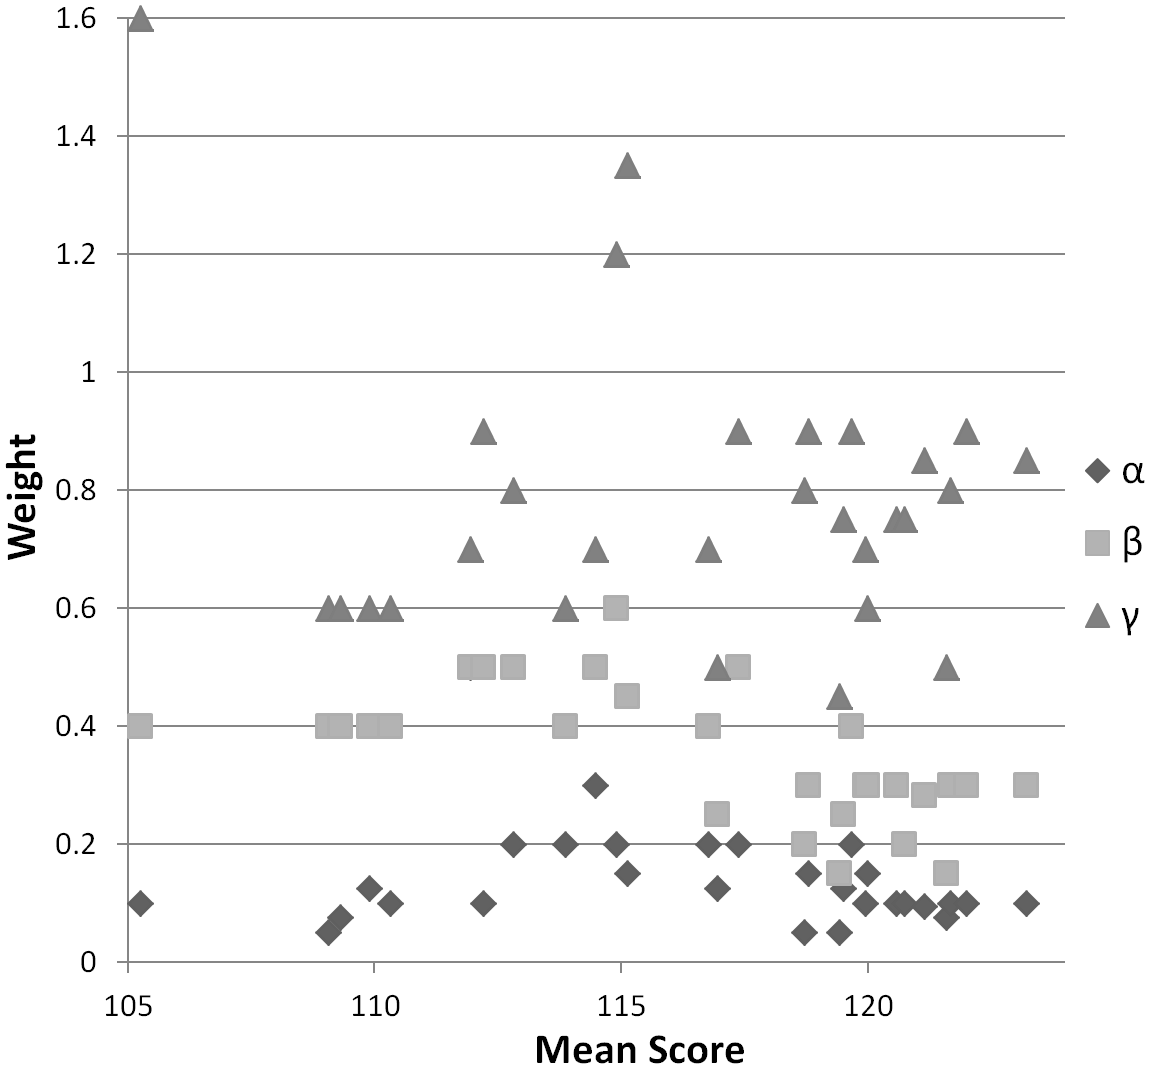
\includegraphics[width=1\linewidth]{images/1-2-3_weights.png}
\end{center}
\caption{$\alpha$, $\beta$, and $\gamma$ for each resulting mean score.}
\label{fig:123weights}
\end{figure}

\begin{figure}[t]
\begin{center}
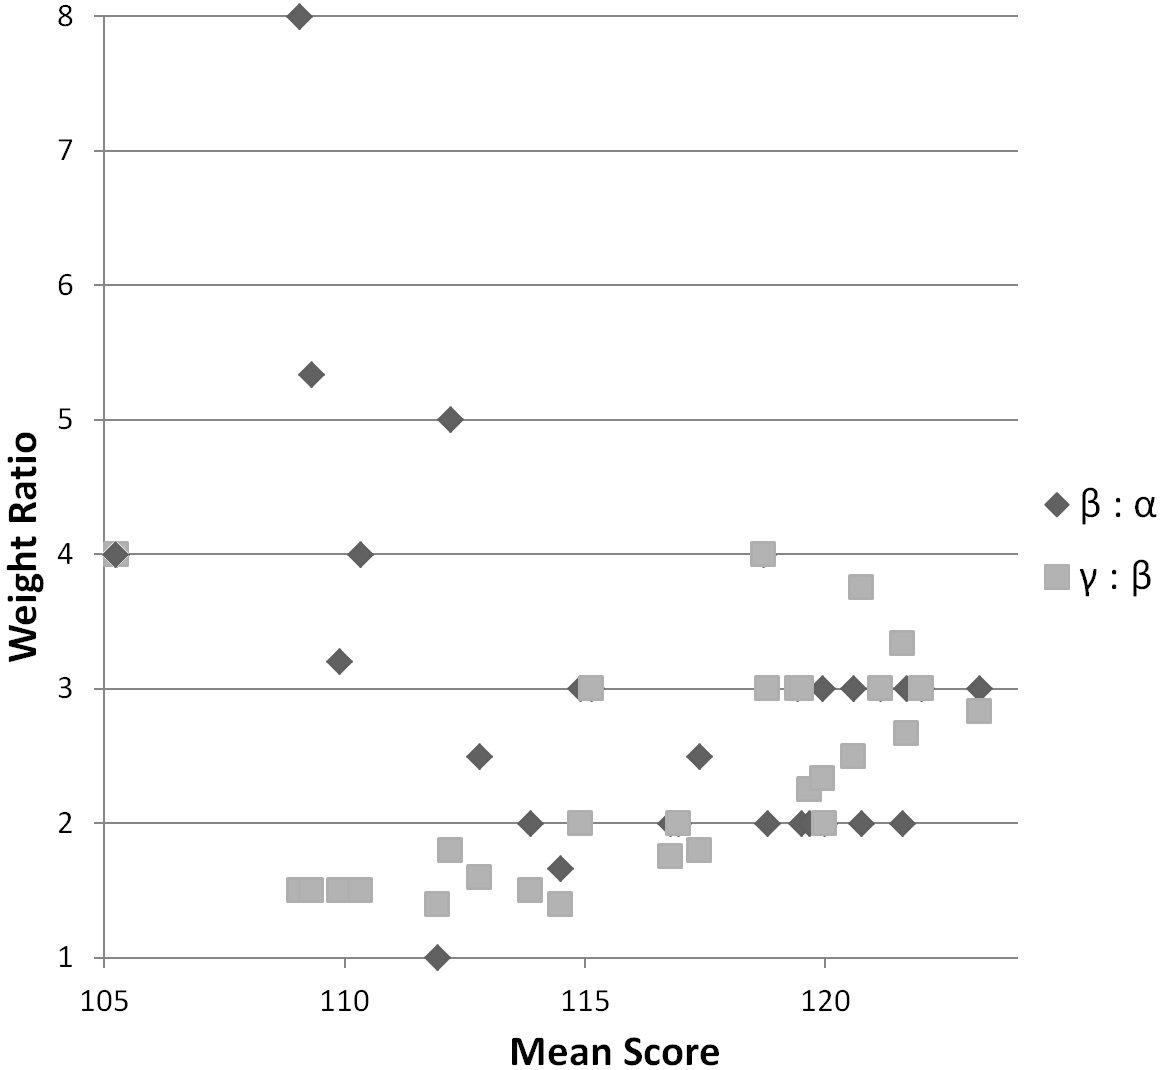
\includegraphics[width=1\linewidth]{images/1-2-3_ratios.png}
\end{center}
\caption{$\beta:\alpha$ and $\gamma:\beta$ for each resulting mean score.}
\label{fig:123ratios}
\end{figure}

This set of experiments considers further tuning of the heuristic while using prune + UCT selection and best move simulation. Recall that thus far heuristic parameters are fixed at $\alpha = 0.2$, $\beta = 0.4$, and $\gamma = 0.6$ for the weighting given to one-, two-, and three-card hands, respectively. For brevity, we denote this here as $[0.2, 0.4, 0.6]$. This section considers various settings of these parameters. We constrain $\alpha \leq \beta \leq \gamma$, and consider both parameter magnitudes and the ratios $\beta : \alpha$ and $\gamma : \beta$ in selecting experimental settings.

%This can bring new insights into what parameter settings may be more similar than would first appear by considering magnitudes alone, thus leading to hypotheses about what portions of the space should be prioritized for consideration. Having said this, however, recall that four-card hands are evaluated using an entirely different formula. So in fact the magnitudes of $\alpha$, $\beta$, and $\gamma$ do matter as well, rather than just the ratios, because hands with three or fewer cards will be compared not just among themselves but against four- and even five-card hands. So using ratios can be a useful analysis tool, but should not be used to the exclusion of considerations of magnitude.

Figures~\ref{fig:123weights} and \ref{fig:123ratios} show results of these experiments for the American scoring system. For example, with $[0.05, 0.4, 0.6]$, a mean score of 109 was obtained. This corresponds to the three left-most data points in Figure~\ref{fig:123weights}, where vertical placement of the symbols indicates parameter settings, and horizontal placement indicates mean score. In Figure~\ref{fig:123ratios}, since $\beta:\alpha = 8.0$ and $\gamma:\beta = 1.5$ for $[0.05, 0.4, 0.6]$, the two leftmost ratio symbols are at vertical points 8.0 and 1.5.

Note in both figures that the results are fairly scattered on the left side where mean scores are lower, yet somewhat more uniform on the right side where mean scores are higher. This demonstrates a preference for certain parameter settings to obtain the highest scores. For example, in Figure~\ref{fig:123weights}, nearly all higher-scoring players tend to converge towards the highest-scoring player's $[0.1, 0.3, 0.85]$, with stronger convergence in the $\alpha$ and $\beta$ values. Some trends are also visible in Figure~\ref{fig:123ratios}, where the highest-scoring players tend to have both weight ratios around 3. The highest scoring player attains a mean score of 123 in the American scoring system (row (12) of Table~\ref{tbl:SelSim}). The \mbox{*} next to the score in the table indicates $[0.1, 0.3, 0.85]$ rather than $[0.2, 0.4, 0.6]$. This is a strong improvement over the 113 of row (9).

We now return to prune + UCT selection, which seemed ineffective in the results of the previous section. Row (10) shows that prune + UCT selection with $[0.1, 0.3, 0.85]$ attains a 94. This is compared to the 91 (row (8)) with $[0.2, 0.4, 0.6]$, and the 92 (row (1)) of standard MCTS. Similarly, best move simulation with $[0.1, 0.3, 0.85]$ scores 118 (row (11)), showing further improvement over the 112 (row (6)) with $[0.2, 0.4, 0.6]$. These experiments demonstrate that both prune + UCT selection and best move simulation can be improved and are worthwhile after tuning to the domain.

%{\bf SAB But we have more experiments here too, right? Some that ran for an extra long time, and some on the 4-card weight. What important conclusions could we draw from those if we wrote them up carefully?}

%{\bf SAB ***** Make sure we address the different scoring systems - does system perform well with them?}

%{\bf SAB Maybe a section about broader conclusions to draw... (not just in PPS)}

%%%%%%%%%%%%%%%%%%%%%%%%%%%%%%%%%%%%%%%%%%%%%%%%%%%%%%%%%
\section{Conclusion and Future Work}

This paper has described the application of MCTS to Parameterized Poker Squares. Experiments show that with carefully-tuned domain knowledge, pruning in selection and a best move simulation lead to significant improvements in performance. These improvements overcome the added cost of these strategies, particularly in simulation.

This work generates a number of interesting follow-up questions for further research. Further experiments on the pruning threshold policy (including the $\delta$ value) may tune the pruning procedure for even more gains. The heuristic could also be explored further in comparing 3-card and 4-card hand evaluations. The experiments on $C_p$ values warrant further exploration and perhaps generalization to other games in the hope of identifying best practices when squashing to $[0,1]$ is challenging. Experiments on other scoring systems suggest the results of this paper are very applicable in general, but minor variations exist that could be exploited in further tuning. Finally, given the significant time-constraints of the PPS player described here, significant gains may be found in applications of parallelism.

\bibliographystyle{aaai}
\bibliography{PPS-Paper}

\end{document}
